\frame{\titlepage}
{
\usebackgroundtemplate{
    \rule{0pt}{\paperheight}
    \hspace*{\paperwidth}
    \makebox[0pt][r]{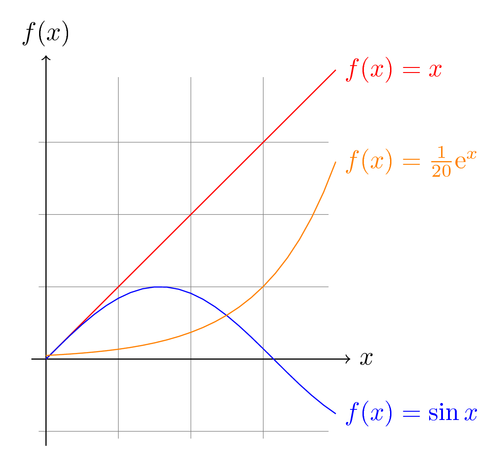
\includegraphics[width=.4\linewidth]{../Figures/ex3.png}}
}
\frame{\frametitle{Содержание}\tableofcontents}
}

\section{Введение, история создания}

\begin{frame}{\TeX~--- творение Дональда Кнута}
    \begin{columns}
        \column{.4\textwidth}
        \centering
        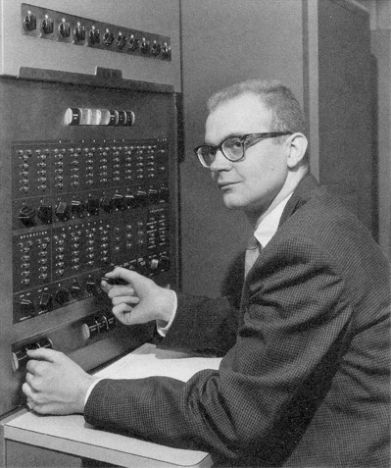
\includegraphics[width=1\linewidth]{../Figures/knut.jpg}

        Дональд Кнут
        \column{.6\textwidth}
        \TeX~--- система компьютерной вёрстки типографии
        \begin{itemize}
            \pause\item греч. $\boldsymbol{\tau\varepsilon\chi\nu\eta}$ --- ``искусство'', ``мастерство'';
            \pause\item METAFONT.
        \end{itemize}
    \end{columns}
\end{frame}

\begin{frame}{\LaTeX, Лесли Лэмпорт}
    \begin{columns}
        \column{.4\textwidth}
        \centering
        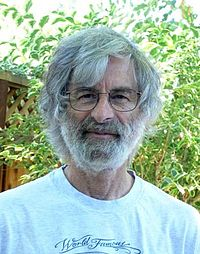
\includegraphics[width=1\linewidth]{../Figures/leslie.jpg}

        Лесли Лэмпорт
        \column{.6\textwidth}
        \LaTeX~--- система верстки научных математических документов
    \end{columns}
\end{frame}

\begin{frame}{Сравнение качества WYSIWYG и \LaTeX}
    \centering
    
\includegraphics[width=.3\linewidth]{../Figures/quality.png}

    Сверху --- \LaTeX.
\end{frame}

\begin{frame}{История создания \TeX}
    \begin{columns}
        \column{.4\textwidth}
        \centering
        
\includegraphics[width=1\linewidth]{../Figures/art.jpg}
        \column{.6\textwidth}
        \begin{itemize}
            \pause\item 1962 -- 1969 --- ``Искусство программирования'';
            \pause\item 1967 --- второе издание;
            \pause\item 1977 --- новые оттиски;
            \pause\item 13 мая 1977 --- рождение \TeX;
            \pause\item текущая версия \TeX~--- 3.14159265;
            \pause\item ядро \TeX~--- язык низкоуровневой разметки.
        \end{itemize}
    \end{columns}
\end{frame}

\begin{frame}{История \LaTeX}
    \begin{columns}
        \column{.4\textwidth}
        \centering
        
\includegraphics[width=1\linewidth]{../Figures/artlatex.jpg}

        \LaTeX~--- макропакет системы \TeX
        \column{.6\textwidth}
        \begin{itemize}
            \pause\item 1984 --- первая версия выпущена Лесли Лэмпортом;
            \pause\item произносится как ``латех'', ``лейтех'', ``латек'' или ``лейтек'';
            \pause\item AMS-\TeX, Xym\TeX, xypic, beamer;
            \pause\item CTAN.
        \end{itemize}
    \end{columns}
\end{frame}

\begin{frame}{CTAN}
    \begin{columns}
        \column{.4\textwidth}
        \centering
        
\includegraphics[width=1\linewidth]{../Figures/ctan.png}

        Comprehensive \TeX Archive Network
        \column{.6\textwidth}
        \begin{itemize}
            \pause\item CTAN --- всеобъемлющая сеть архивов \TeX;
            \pause\item возник спонтанно;
            \pause\item 4783 пакета, 2225 авторов;
            \pause\item от химических формул до принципиальных схем.
        \end{itemize}
    \end{columns}
\end{frame}

\section{Сравнение \LaTeX~и текстовых процессоров} %Зачем это нужно

\defverbatim[colored,width=.5\textwidth]\equationExample{
    \begin{minted}[breaklines,gobble=8,fontsize=\small]{latex}
        \sum\limits_{k=1}^{\sigma} f_k(x,u) = \int\limits_a^x \frac{dx}{\sqrt{x^2 + a^2}}
    \end{minted}
}

\begin{frame}{Плюсы \LaTeX}
    \begin{columns}
        \column{.5\textwidth}
        \centering
        \only<1,5>{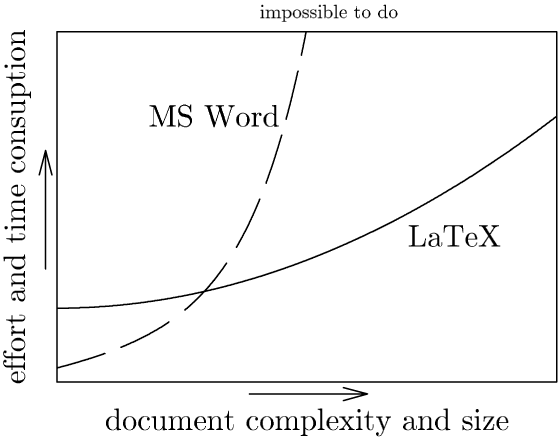
\includegraphics[width=1\linewidth]{../Figures/graph.png}}
        \only<2>{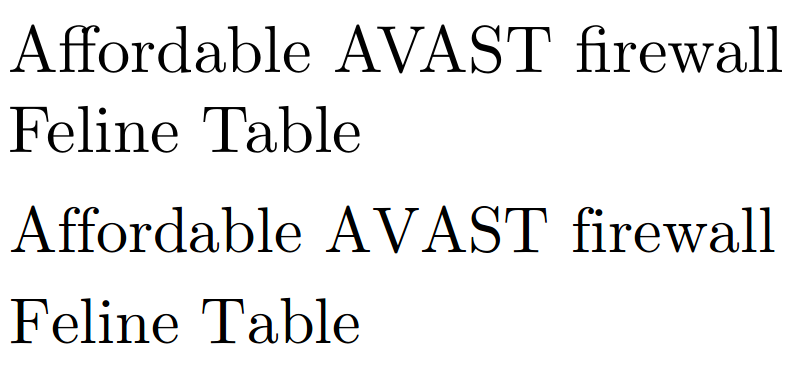
\includegraphics[width=1\linewidth]{../Figures/difference.png}}
        \only<3>{
\includegraphics[width=1\linewidth]{../Figures/free.png}}
        \only<4>{
            \equationExample

            $\sum\limits_{k=1}^{\sigma} f_k(x,u) = \int\limits_a^x \frac{dx}{\sqrt{x^2 + a^2}}$.
        }
        \only<6>{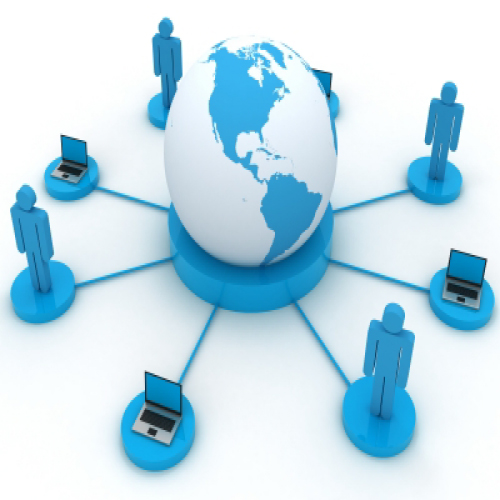
\includegraphics[width=1\linewidth]{../Figures/collective.jpg}}
        \only<7>{
\includegraphics[width=1\linewidth]{../Figures/portability.png}}
        \only<8>{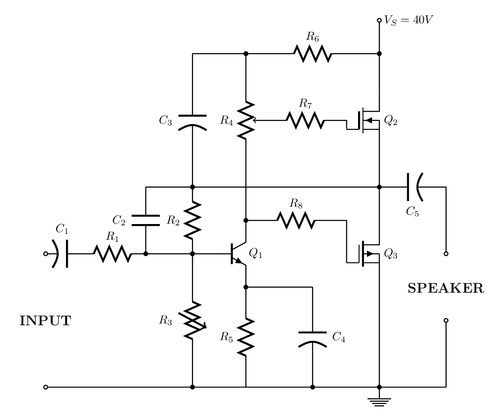
\includegraphics[width=1\linewidth]{../Figures/ex1.png}}
        \column{.5\textwidth}
        \begin{itemize}
            \pause\item качество выходного документа;
            \pause\item бесплатность и открытость;
            \pause\item удобство (нумерация, содержание, набор формул);
            \pause\item концентрация на содержимом;
            \pause\item возможность коллективной работы;
            \pause\item переносимость;
            \pause\item программируемые графики и схемы.
        \end{itemize}
    \end{columns}
\end{frame}

\begin{frame}{Когда не нужно использовать \LaTeX}
    \begin{columns}
        \column{.4\textwidth}
        \centering
        \only<1>{
\includegraphics[width=1\linewidth]{../Figures/stop.jpg}}
        \only<2>{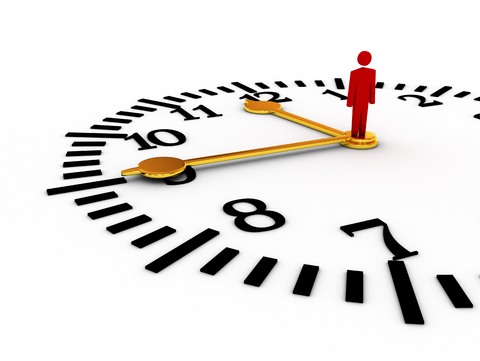
\includegraphics[width=1\linewidth]{../Figures/time.jpg}}
        \only<3>{
\includegraphics[width=1\linewidth]{../Figures/word.png}}
        \only<4>{
\includegraphics[width=1\linewidth]{../Figures/design.png}}
        \column{.6\textwidth}
        \begin{itemize}
            \pause\item когда нет времени его учить;
            \pause\item если документ уже написан в текстовом процессоре;
            \pause\item если необходим креативный дизайн.
        \end{itemize}
    \end{columns}
\end{frame}

\defverbatim[colored,width=.6\textwidth]\enumerateExample{
    \begin{minted}[breaklines,gobble=8,fontsize=\small]{latex}
        \begin{enumerate}
            \item Первый пункт.
            \item Второй пункт.
        \end{enumerate}
    \end{minted}
}

\defverbatim[colored,width=.6\textwidth]\enumerateUse{
    \begin{minted}[breaklines,gobble=8,fontsize=\small]{latex}
        \usepackage{enumerate}
    \end{minted}
}

\begin{frame}{Возможности \LaTeX}
    \begin{columns}
        \column{.6\textwidth}
        \centering
        \enumerateExample
        \column{.4\textwidth}
        \begin{enumerate}
            \item Первый пункт.
            \item Второй пункт.
        \end{enumerate}
    \end{columns}
    \vfill
    \centering
    \begin{minipage}{.4\textwidth}
        \enumerateUse
    \end{minipage}
\end{frame}

\section{Примеры использования, структура документа}

\defverbatim[colored]\pictureExample{
    \begin{minted}[breaklines,gobble=8,fontsize=\small]{latex}
        \begin{figure}[ht]
            \subcaptionbox{}{
                $\alpha = \left| \begin{matrix}
                    1 & 0 & 0\\
                    0 & 1 & 1\\
                    0 & 0 & 1
                \end{matrix} \right|.$
            }
            \qquad
            \subcaptionbox{}{
                \includegraphics[width=.2\linewidth]{fig.png}
            }
            \caption{Пример рисунка (а) матрица, описанная при помощи \LaTeX; (б) картинка}
        \end{figure}
    \end{minted}
}

\begin{frame}{Примеры использования}
    \pictureExample
\end{frame}

\begin{frame}{Результат}
    \begin{figure}[ht]
        \subcaptionbox{}{
            $\alpha = \left| \begin{matrix}
                1 & 0 & 0\\
                0 & 1 & 1\\
                0 & 0 & 1
            \end{matrix} \right|.$
        }
        \qquad
        \subcaptionbox{}{
            
\includegraphics[width=.2\linewidth]{../Figures/somepicture.png}
        }
        \caption{Пример рисунка (а) матрица, описанная при помощи \LaTeX; (б) картинка}
    \end{figure}
\end{frame}

\defverbatim[colored]\equExample{
    \begin{minted}[gobble=8,fontsize=\small]{latex}
        Ссылка на формулу --- формула \ref{eq:some}.

        \begin{equation}
            \int\limits_0^\pi x dx = \textup{\Huge{?}}
            \label{eq:some}
        \end{equation}
    \end{minted}
}

\begin{frame}{Пример формулы}
    \equExample

    Ссылка на формулу --- формула \ref{eq:some}.

    \begin{equation}
        \int\limits_0^\pi x dx = \textup{\Huge{?}}
        \label{eq:some}
    \end{equation}
\end{frame}

\defverbatim[colored]\structureEx{
    \begin{minted}[gobble=8,fontsize=\small]{latex}
        \documentclass{article}

        \begin{document}
        %Здесь располагается тело документа
        \end{document}
    \end{minted}
    \vfill
    \inputminted[breaklines,firstline=1,lastline=1,fontsize=\small]{latex}{../../../preamble.tex}
    \vfill
    \inputminted[fontsize=\small]{latex}{../../main.tex}
    \vfill
    \mint[fontsize=\small]{latex}|\section*{Введение}|
}

\begin{frame}{Структура документа}
    \structureEx
\end{frame}

\begin{frame}{Структура директорий}
    \centering
    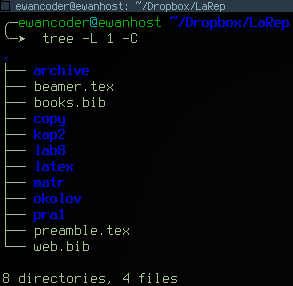
\includegraphics[width=.4\linewidth]{../Figures/tree.png}
    \qquad
    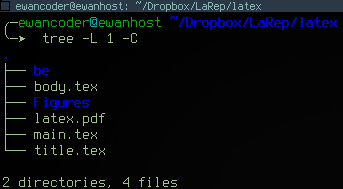
\includegraphics[width=.4\linewidth]{../Figures/tree2.png}
\end{frame}

\defverbatim[colored]\preambleEx{
    \inputminted[breaklines,firstline=1,lastline=6,fontsize=\small]{latex}{../../../preamble.tex}
    \mint{latex}|Пример - трех -- видов --- тире|
    \mint{latex}|''Неправильные`` кавычки|
}

\begin{frame}{Начало преамбулы}
    \preambleEx
    ''Неправильные`` кавычки

    Пример - трех -- видов --- тире
\end{frame}

\section{Наиболее популярные пакеты \LaTeX}

\defverbatim[colored]\packOne{
    \inputminted[breaklines,firstline=8,lastline=15,fontsize=\small]{latex}{../../../preamble.tex}
}
\begin{frame}{Стандартные пакеты настройки содержимого}
    \packOne
\end{frame}

\defverbatim[colored]\packTwo{
    \inputminted[breaklines,firstline=17,lastline=21,fontsize=\small]{latex}{../../../preamble.tex}
}
\defverbatim[colored]\packThree{
    \inputminted[breaklines,firstline=23,lastline=27,fontsize=\small]{latex}{../../../preamble.tex}
}
\begin{frame}{Стандартные пакеты настройки содержимого}
    \packTwo
    \vfill
    \packThree
\end{frame}

\begin{frame}{Экзотические пакеты}
    \centering
    \begin{itemize}
        \pause\item tikz
        \pause\item beamer
        \pause\item dissert
        \pause\item karnaugh
    \end{itemize}
\end{frame}

\begin{frame}{TIKZ}
    \begin{figure}[!ht]
        \subcaptionbox{}{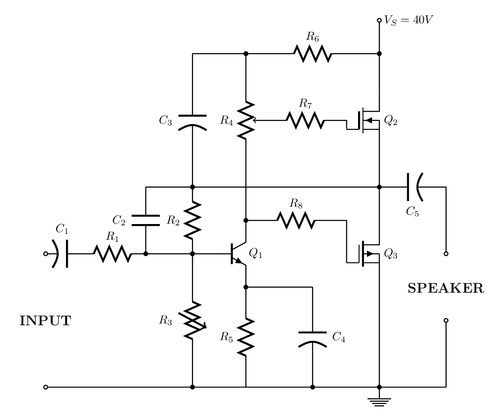
\includegraphics[width=.3\linewidth]{../Figures/ex1.png}}
        \subcaptionbox{}{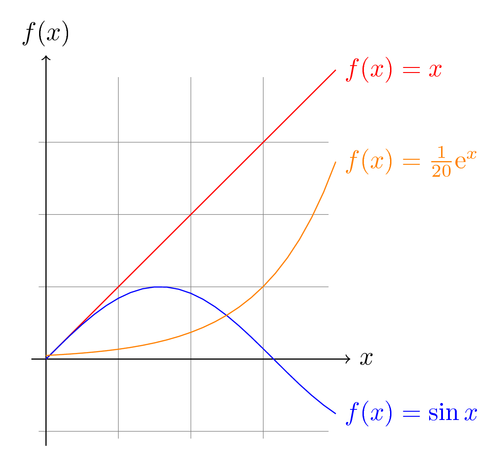
\includegraphics[width=.3\linewidth]{../Figures/ex3.png}}
        \subcaptionbox{}{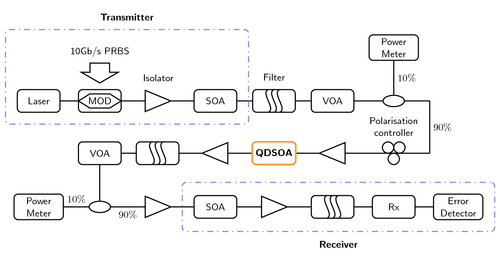
\includegraphics[width=.3\linewidth]{../Figures/ex2.png}}
        
        Примеры tikz (а) электрическая принципиальная схема; (б) график; (в) блок-схема
    \end{figure}
\end{frame}

\section{Библиография}

\begin{frame}{Недостатки встроенной библиографии}
    \centering
    \begin{itemize}
        \pause\item неверный порядок источников;
        \pause\item нет возможности поменять стиль;
        \pause\item нельзя использовать одни и те же источники в нескольких документах.
    \end{itemize}
\end{frame}

\defverbatim[colored]\webBib{
    \mint[fontsize=\small]{latex}|\bibliography{../web}|
    \vfill
    \inputminted[breaklines,firstline=1,lastline=7,fontsize=\small]{latex}{../../../web.bib}
}

\begin{frame}{Альтернатива --- BiB\TeX}
    \webBib
\end{frame}

\section{Редактирование и компиляция}

\begin{frame}{Редакторы \LaTeX}
    \begin{columns}
        \column{.4\textwidth}
        \centering
        
\includegraphics[width=.4\linewidth]{../Figures/vim.png}

        
\includegraphics[width=.4\linewidth]{../Figures/texstudio.png}
        \column{.6\textwidth}
        \begin{itemize}
            \pause\item VIM --- блокнот с богатыми возможностями;
            \pause\item \TeX studio --- мощная кроссплатформенная IDE \LaTeX.
        \end{itemize}
    \end{columns}
\end{frame}

\defverbatim[colored]\compileEx{
    \begin{minted}[gobble=8,fontsize=\small]{latex}
        pdflatex main
        bibtex main
        pdflatex main
        pdflatex main
    \end{minted}
}

\begin{frame}{Изъяны компиляции}
    \compileEx
    \vfill
    \pause Xe\TeX, Xe\LaTeX~--- альтернативы \LaTeX.
\end{frame}

\defverbatim[colored]\beamerEx{
    \inputminted[breaklines,firstline=3,lastline=3,fontsize=\small]{latex}{/home/ewancoder/Dropbox/LaRep/beamer.tex}
    \vfill
    \begin{minted}[gobble=8,fontsize=\small]{latex}
        \begin{frame}
            \begin{itemize}
                \pause\item Первый пункт;
                \pause\item Второй пункт;
                \pause\item Третий пункт.
            \end{itemize}
        \end{frame}
    \end{minted}
}

\section{Создание презентаций средствами \LaTeX}

\begin{frame}{Создание презентаций средствами \LaTeX}
    \beamerEx
\end{frame}

\section{Заключение}

{
\usebackgroundtemplate{
\includegraphics[width=\paperwidth]{../Figures/thanks.png}}
\begin{frame}
    \centering
    \vfill
    \vfill
    \large{Презентация была создана средствами {\LaTeX} и Beamer}
\end{frame}
}
